%\documentclass[sigplan,screen]{acmart}
\documentclass[newfonts=false,format=sigconf,10pt,letterpaper]{acmart}

\usepackage{xspace}
\usepackage{graphicx}
\usepackage{subcaption}
\usepackage[english]{babel}
\usepackage{textcomp}
\usepackage{times}
\usepackage{amsmath}
\usepackage{setspace}
\usepackage[inline]{enumitem}

%%%%%%%%%%%%%%%%%%%%% Commands from prev version
\usepackage[utf8]{inputenc}
%\usepackage[numbers]{natbib}
% \usepackage[noadjust]{cite}

%\renewcommand{\citedash}{--}  
\newlist{inlinelist}{enumerate*}{1}
\setlist[inlinelist]{label=(\arabic*)}
\newlist{romanlist}{enumerate*}{1}
\setlist[romanlist]{label=(\roman*)}


\providecommand{\vs}{vs. }
\providecommand{\ie}{\emph{i.e.,} }
\providecommand{\eg}{\emph{e.g.,} }
\providecommand{\cf}{\emph{cf.,} }
\providecommand{\etc}{\emph{etc.} }

\newcommand{\sockets}{Berkeley sockets\xspace}
\newcommand{\proxies}{relays\xspace}
\newcommand{\reconn}{pre-established connections\xspace}
\newcommand{\usec}{$\mu$sec\xspace}

\newcommand{\T}[1]{\smallskip\noindent\textbf{#1}}
\newcommand{\oursys}{KTCP\xspace}
\newcommand{\relays}{CBN routers\xspace}
\newcommand{\relay}{CBN router\xspace}
%a macro for defining a new variable in the document
\newcommand{\newVar}[2]{\newcommand{#1}{\ensuremath{#2}\xspace}}
%%%%%%%%%%%%%%%%%%%%%%%%%%%%%%%%%%%%%%%
\newVar{\rc}{R_C}
\newVar{\rs}{R_S}
\newVar{\rmid}{R_M}
\newVar{\rtt}{T}

\newcommand{\mycomm}[3]{{\footnotesize{{\color{#2} \textbf{[#1: #3]}}}}}
%    \newcommand{\mycomm}[3]{}
%define your comment NAME and COLOR here
\newcommand{\IK}[1]{\mycomm{IK}{blue}{#1}}
%%%%%%%%%%%%%%%%%%%%%%%%%%%%%%%%%%%%%%%%%%%%%%%

\title{Kernels of Splitting TCP in the Clouds}
\author{Markuze Alex}
\email{amarkuze@vmware.com}
\affiliation{%
  \institution{VMware Research}
  \country{Israel}
}

\author{Bergman Aran}
\email{bergmana@vmware.com}
\affiliation{%
  \institution{VMware Research}
  \country{Israel}
}

\author{Dar Chen}
\email{cdoar@vmware.com}
\affiliation{%
  \institution{VMware Research}
  \country{Israel}
}

\author{Israel Cidon}
\email{icidon@vmware.com}
\affiliation{%
  \institution{VMware Research}
  \country{Palo Alto}
}
%%% potentially enable (i.e. remove the disable command) for the fields below in the camera-ready version          
\settopmatter{printacmref=false}
%\settopmatter{printfolios=false,printacmref=false} %numbers the pages; remove the ugly ACM reference
   	  \setcopyright{none}
\renewcommand\footnotetextcopyrightpermission[1]{} % removes footnote with conference information in first column
\pagestyle{plain} % removes running headers
\date{January 2019}

\begin{document}

\begin{abstract}
The \emph{Cloudified Business Network}(CBN) project~\cite{Elastic, CDD} constructs a global overlay network across public clouds. CBN interconnects geographically-dispersed corporate datacenters and branches. CBN leverages the global geographical spread of public clouds and their vast compute and networking infrastructure.
Clients using CBN could see improvements in download times sometimes by orders of magnitude. The main ingredient in improving network performance was shown to be the split TCP technique~\cite{CDD, }. 
%\IK{BTW you sell this as being about CBN only, but maybe you want to state that it's more general and could be used in a vast range of VMware products that could rely on TCP split, eg for VM migration?} 
Unfortunately, the available TCP split solutions incur a penalty on connection time, and actually hurt the performance of short flows. In addition, all available TCP split implementations are in user-space, and thus have two expensive system calls per forwarded segment. The redundant system calls hurt server performance and limit the scalability of such solutions.
\newline
This paper describes \oursys, a Linux Kernel module written for CBN. \IK{In the next sentences: 1. I suggest moving all sentences like ``our goal was..." to the first paragraph and merge into one of the sentences that state ``Current TCP split solutions also do not..." 2. I was missing 1-2 sentences about the algorithms/techniques/novelty in the result.} When designing \oursys our goal was to create a reliable tool that could be safely used in an industry grade product.  \oursys is built with well trusted and tested "off-the-shelf" components. At the same time we were aiming to  minimize and effectively eliminate any overheads of establishing the split TCP connection. \oursys is built for CBN multi-tenant environment and designed to linearly scale on multi-core systems. \IK{Is this new? hard?} We show how \oursys is able to increase the network bandwidth and minimize the connection \emph{latency} close to the physically possible. \IK{you tell us that it achieves many things in hindsight, but haven't prepared us by telling us from the start why we care about them}

\end{abstract}

\maketitle

\section{Introduction}
\section{laying pipes in the clouds}\label{sec:rate-control}

\subsection{The Dream Network Pipe}\label{subsec:dream-pipe}

\begin{figure*}[!t]
  \centering
    \begin{subfigure}{0.65\columnwidth}
  \centering
  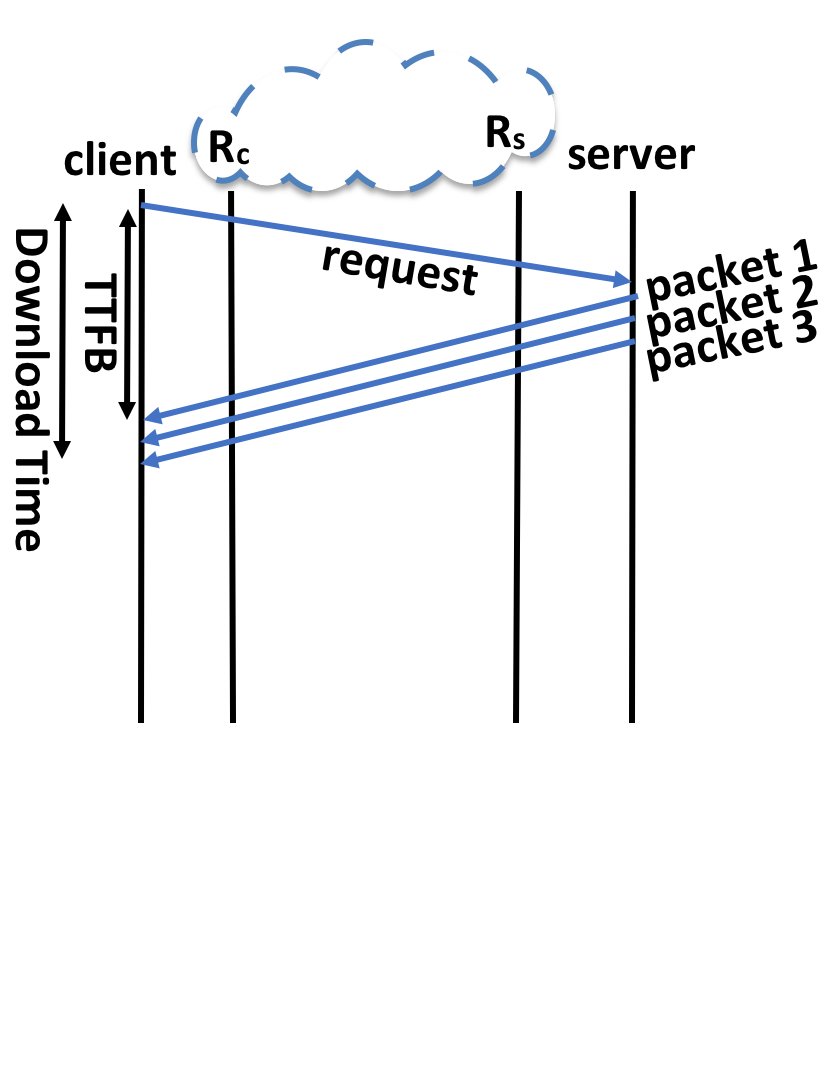
\includegraphics[width=\columnwidth]{figures/ideal.png}
    \caption{Ideal protocol-free transmission.}
    \label{fig:ideal}
\end{subfigure}    \centering
\begin{subfigure}{0.65\columnwidth}
  \centering
  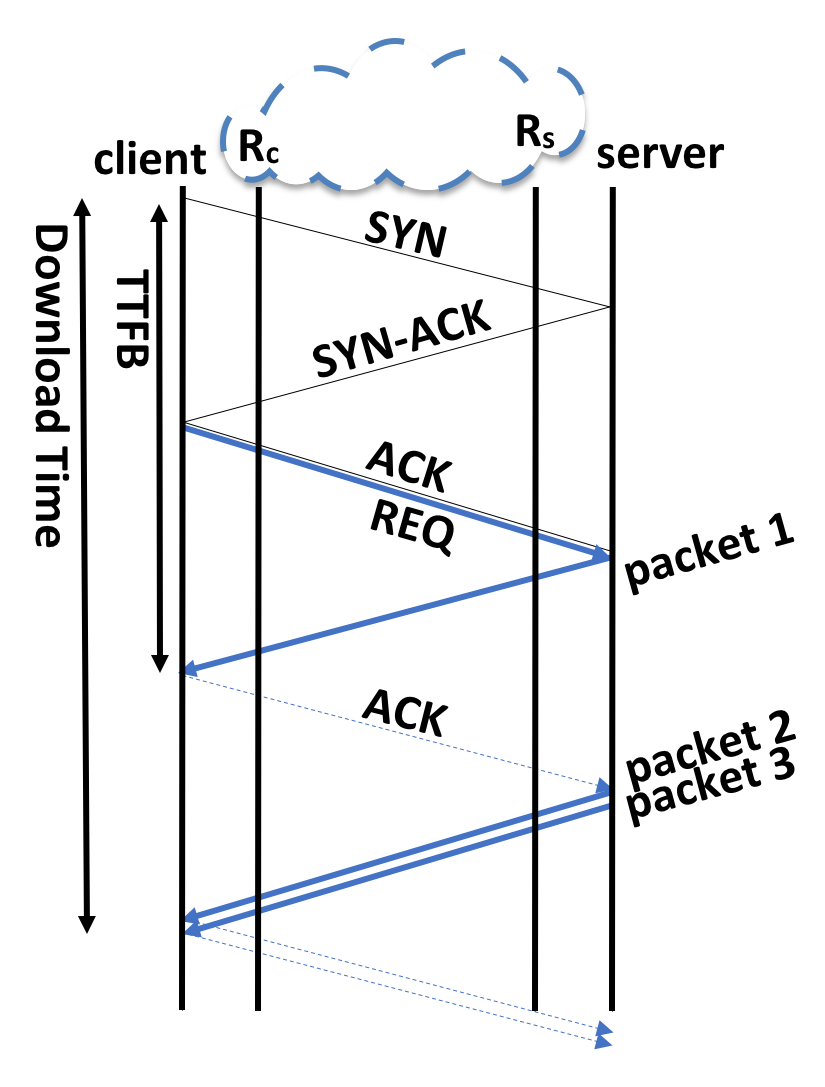
\includegraphics[width=\columnwidth]{figures/e2e.png}%test1.pdf}
    \caption{End-to-end through the Internet (or cloud).} \label{fig:e2e}
\end{subfigure}    \centering
\begin{subfigure}{0.65\columnwidth}
  \centering
  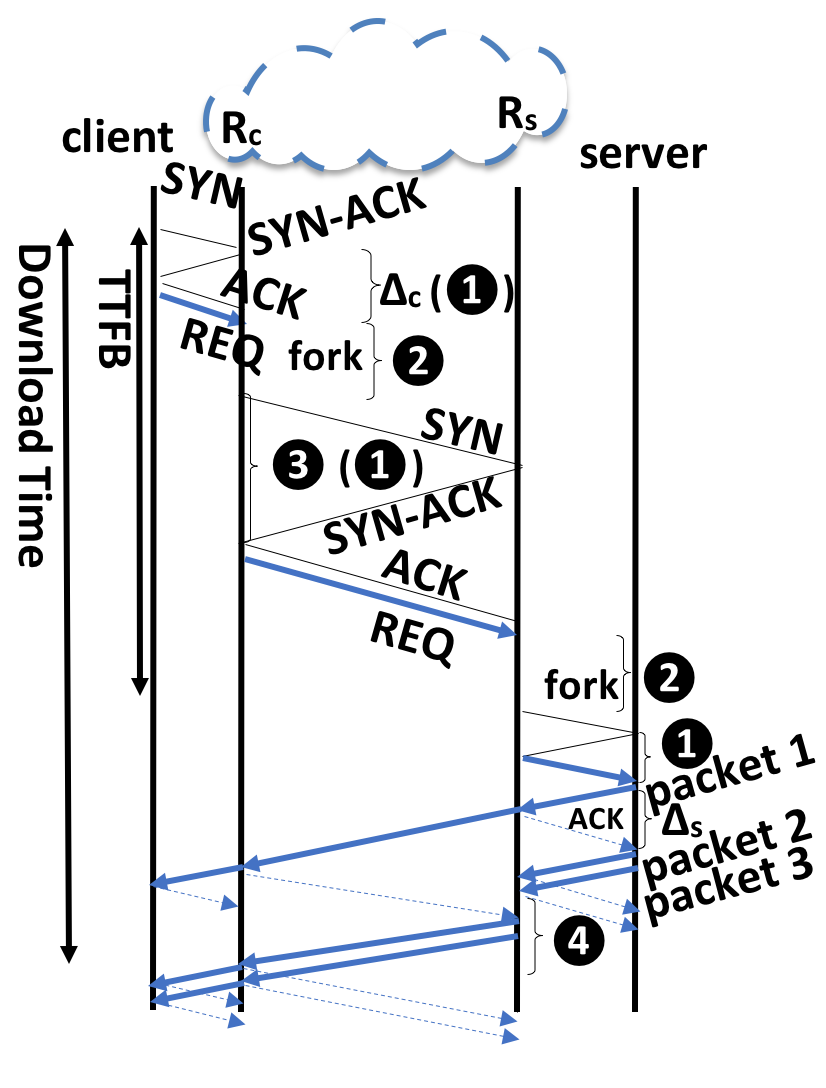
\includegraphics[width=\columnwidth,clip]{figures/split.png}
    \caption{Simple TCP cloud split.} \label{fig:baseline}
\end{subfigure}
%  \centering
% \begin{subfigure}{0.6\columnwidth}
%   \centering
%   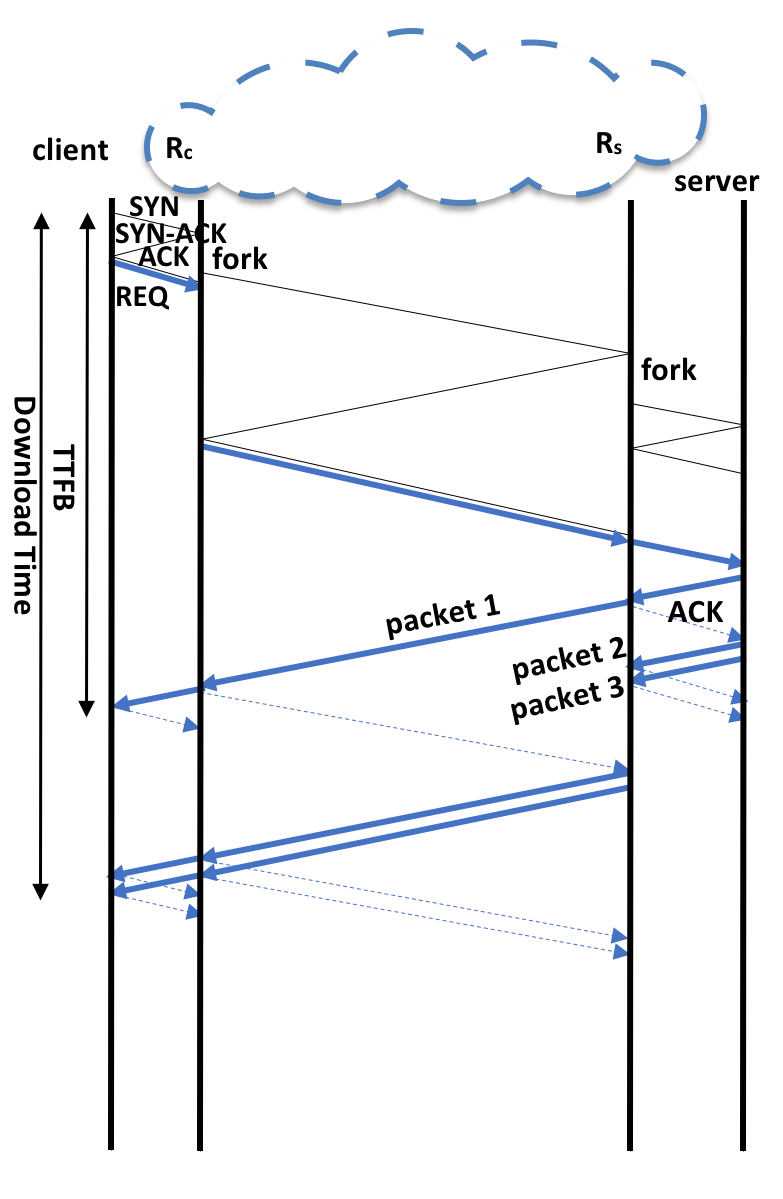
\includegraphics[width=\columnwidth]{figures/early-syn.png}
%     \caption{Early-SYN.} \label{fig:early-syn}
% \end{subfigure}
    \caption{Illustrated comparison of the considered baseline data transmission methods. Suppose, for simplicity of exposition, that the client requests three MSS-sized packets using HTTP over TCP, that the initial TCP window size is one MSS, and that there are no losses.\\ \textit{(a)} In an ideal clean-slate world, the request for packets would go through directly, triggering the transmission of all response packets. The time-to-first-byte (TTFB) is just one round-trip time (RTT), the lowest possible TTFB. The download time is barely higher.\\ \textit{(b)} End-to-end TCP transmission first requires the establishment of an end-to-end connection, adding one RTT to the ideal finish time. Waiting one RTT for the first ACK further delays the download. \\ \textit{(c)} The baseline strategy of Section~\ref{sec:ocd-baseline} decreases the ACK times for longer files, but introduces new delays such as thread fork delays in the connection. This explains why the Baseline is less efficient for small files. We later revisit all the delays that appear beyond those of the ideal transmission (Figure~\ref{fig:oursys-improvements}). We show how to address the delays marked (1)-(4), but are left with delays $\Delta_c$ and $\Delta_s$ on the client and server sides, respectively.  }
\end{figure*}

\begin{figure*}[!t]
  \centering
    \begin{subfigure}{0.48\columnwidth}
  \centering
  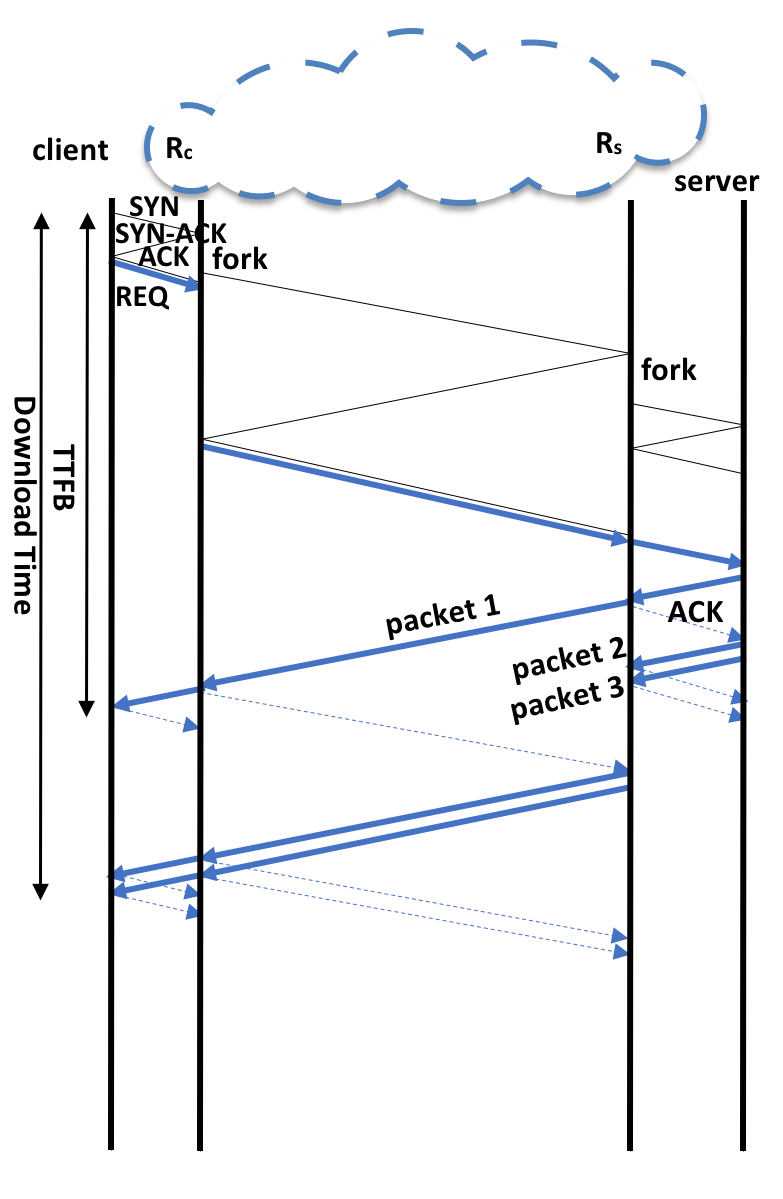
\includegraphics[width=\columnwidth]{figures/early-syn.png}
    \caption{Early-SYN.}
    \label{fig:early-syn}
\end{subfigure}    \centering
\begin{subfigure}{0.48\columnwidth}
  \centering
  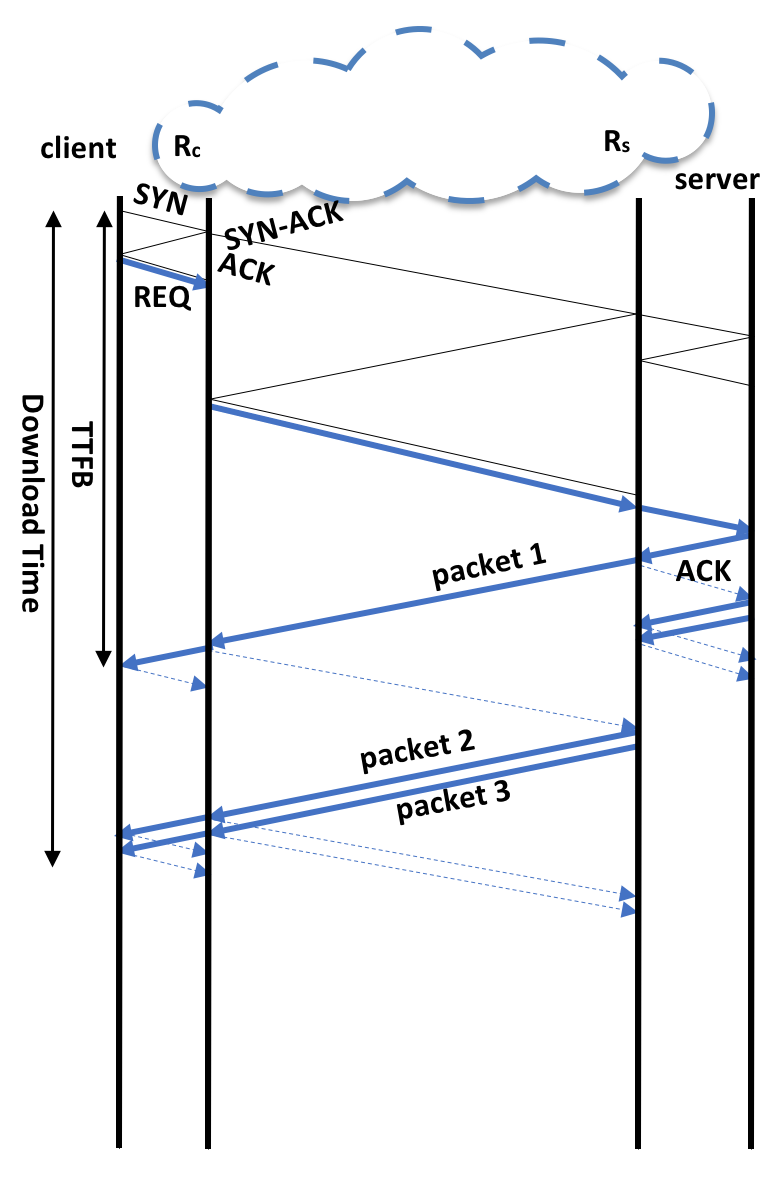
\includegraphics[width=\columnwidth]{figures/thread.png}
    \caption{Thread pool.} \label{fig:thread-pool}
\end{subfigure}    \centering
\begin{subfigure}{0.48\columnwidth}
  \centering
  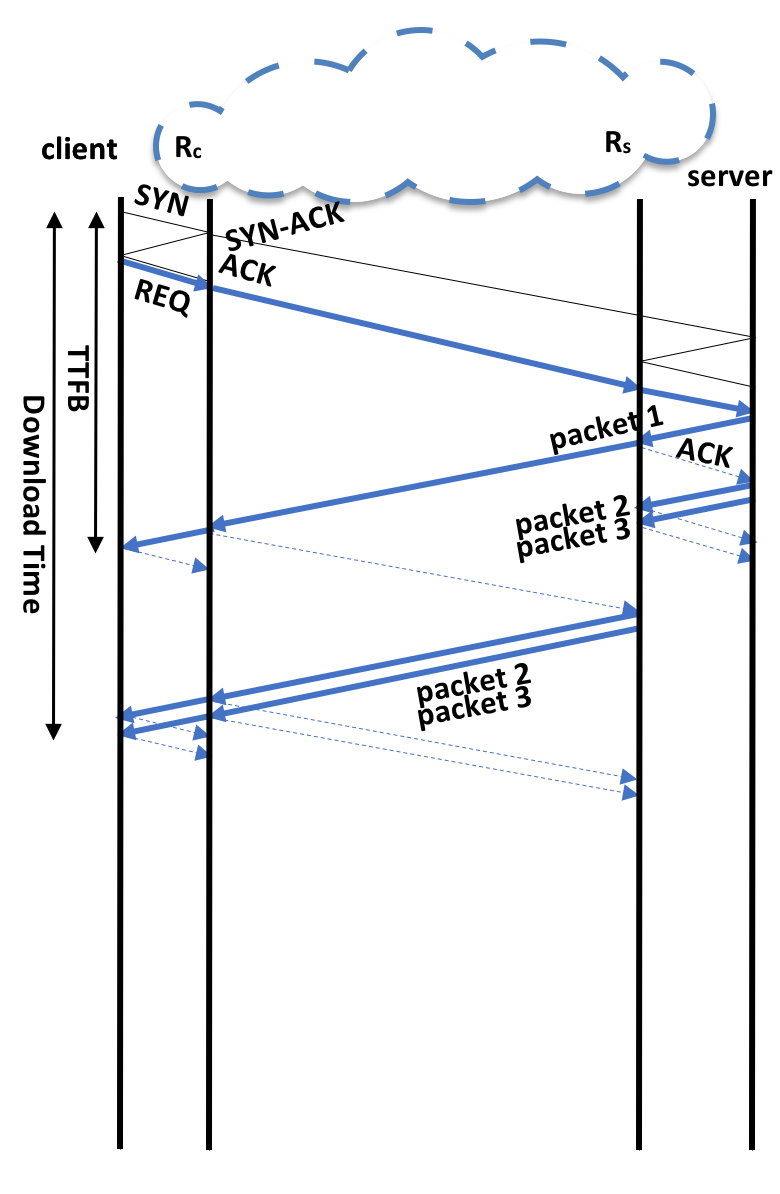
\includegraphics[width=\columnwidth]{figures/connection.png}
    \caption{Connection pool.} \label{fig:connection-pool}
\end{subfigure}     \centering
\begin{subfigure}{0.48\columnwidth}
  \centering
  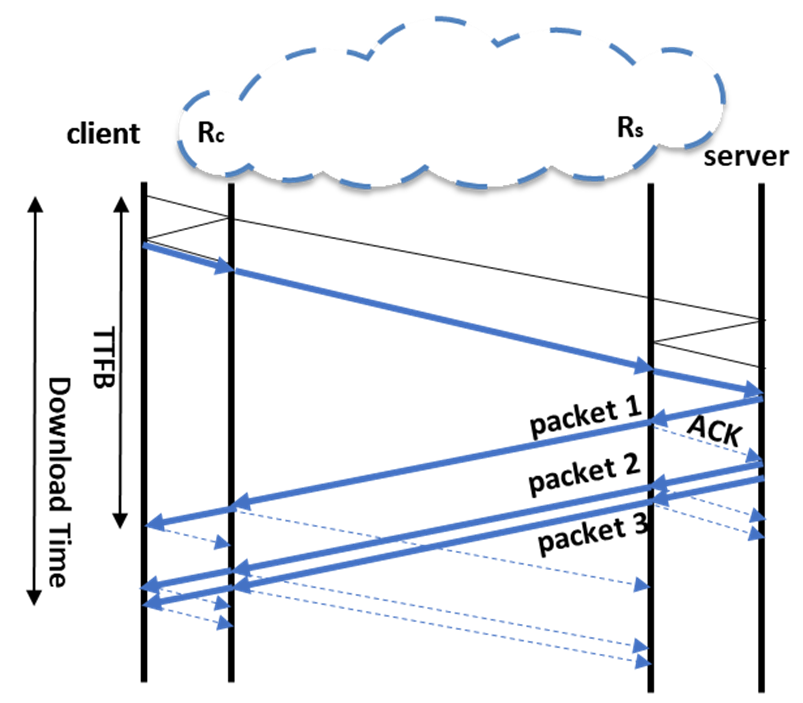
\includegraphics[width=\columnwidth]{figures/turbo.png}
    \caption{Turbo-Start TCP.} \label{fig:turbo-start-tcp}
\end{subfigure}
%  \centering
% \begin{subfigure}{0.6\columnwidth}
%   \centering
%   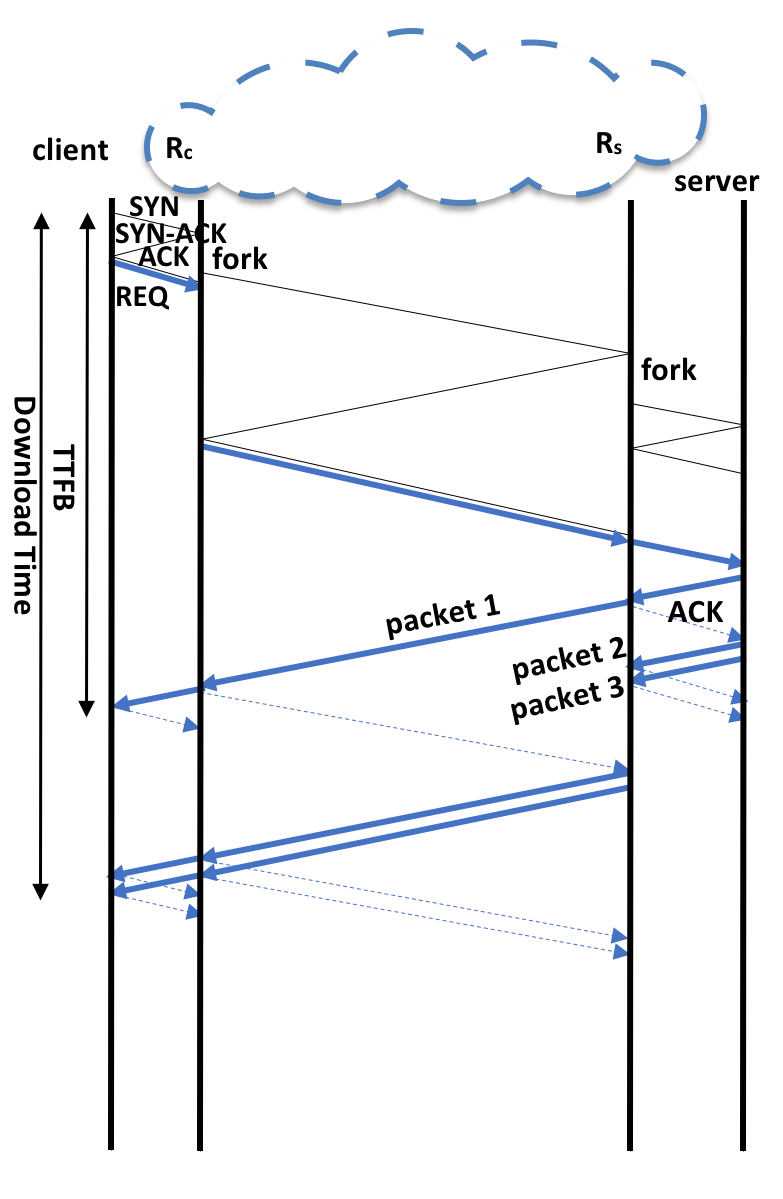
\includegraphics[width=\columnwidth]{figures/early-syn.png}
%     \caption{Early-SYN.} \label{fig:early-syn}
% \end{subfigure}
    \caption{\oursys successive implementation improvements: Using \textit{Early-SYN}, we can remove SYN-ACK and ACK delays (marked as (1) in Figure~\ref{fig:baseline}). Using a \textit{thread pool} removes forks (marked as (2) in Figure~\ref{fig:baseline}). With a \textit{connection pool}, delay (3) in Figure~\ref{fig:baseline} is eliminated. Turbo-Start TCP eliminates delay (4). The two last delays (marked as ``?'' in Figure~\ref{fig:baseline}) that need be removed are delays $\Delta_c$ and $\Delta_s$ on the client and server sides, respectively. As both depend on the client and server parameters, they seem beyond our control. 
    }
    \label{fig:oursys-improvements}
\end{figure*}

%\T{Congestion-less control?} The cloud provides an auto-scaling networking infrastructure with links of virtually-infinite capacity. Like others~\cite{haq2017measuring}, we find that in-cloud paths provide more predictable results than the public Internet, with an order of magnitude lower loss rate. As a result, flows in the cloud will rarely ever encounter congestion. This compels us to rethink the role of congestion control in the cloud. In light of the near-absence of congestion, we essentially want a simple high-rate sending protocol capable of dealing with the very rare loss events, without necessarily backing off. Even flow control is not necessarily needed within the cloud, as clouds can increasingly provide an elastic memory infrastructure~\cite{hotadd,baloon} that can quickly adapt to any receive-buffer temporary load. 

\T{Ideal pipe.} Given the large capacity of the cloud, we wonder how close we could get to an ideal transmissio..
\autoref{fig:ideal} illustrates our fundamental model of an ideal transmission. Importantly, this model reflects a protocol-free, theoretical ideal transmission. Our aim for the remainder of this section is to identify the means for approximating this model in practice. We show in \autoref{fig:e2e} that a classical end-to-end data transfer based on HTTP over TCP falls short 
%\AB{I'm not sure how CC got into this... Some of the delays are not due to congestion control, but due to TCP's operation and design tradeoffs, regardless of CC. Also, should we mention that the diagram assumes HTTP as the transport protocol? (Does it also fit others, like, \eg FTP?)} congestion control falls short 
of this goal. In addition, adding a stop on our  also introduces additional delays with respect to the ideal model. We point out these delays in \autoref{fig:baseline}, and discuss how these delays can be eliminated, so as to come close to our theoretical ideal.

%Realizing rate-control for the cloud could have simply utilized a form of Reliable UDP. To be backwards compatible, we simply used instead a Cubic TCP with an aggressive initial window size.

\subsection{Approximating the Ideal Pipe}\label{sec:approx}

To approximate the ideal data transmission model of Section~\ref{subsec:dream-pipe}, we introduce \textit{\oursys}.
The goal of \oursys is to enhance the OCD Baseline of Section~\ref{sec:ocd-baseline} and provide efficient, delay-free TCP optimization; while utilizing commodity VMs and standard programming APIs. This is done by incorporating four improvements to the baseline strategy, illustrated in Figure~\ref{fig:oursys-improvements}. Together, these four components eliminate the delays marked (1)-(4) in Figure~\ref{fig:baseline}. We next elaborate on each of the four improvements. We discuss the many implementation details involved in realizing \oursys in Section~\ref{sec:design} and provide our open-source code in~\cite{ktcp}.

%\oursys incorporates four improvements to the baseline strategy of Section~\ref{x}, illustrated in Figure~\ref{fig:baseline}. Together, these four improvements eliminate the delays marked (1)-(4) in \ref{fig:oursys-improvements}. We next elaborate on each of the four improvements. We discuss the many implementation details involved in realizing \oursys in Section~\ref{sec:design}.

%\AB{we need to change the order here. Perhaps also in the figure. The Early SYN (named Early SYN Forwarding (ESF) in earlier papers) option cannot be tested on its own, currently (Alex can explain). The first optimization is thread pool, then adding ESF and then changing adding the pre-existing connections...}\IK{Two isues: 1. Noga needs to redo the plots (=numbers in 5c+ full 6a); 2. Early-SYN was done in the past, the other 3 improvements were not, so this order is more logical in this sense...\\ ... that being said, if you/Noga/Eyal are willing to redo the graphs, feel free to go ahead.}


\T{Improvement 1: Early SYN.} In early SYN~\cite{ladiwala,siracusano2016miniproxy}, a SYN packet is sent to the next-hop server as soon as the SYN packet arrives. This is done without waiting for the three-way handshake to complete. \oursys captures this first SYN packet and triggers the start of a new connection. This allows the proxy to establish the two legs of a split connection in parallel. (Note that while this improvement is well-known, to our knowledge the next ones are novel in the context of TCP switching.)

\T{Improvement 2: Thread pool.} 
The creation of new kernel\_threads for each new split connection is time-consuming and adds greatly to the connection jitter. Some outliers may take tens of milliseconds, greatly hurting performance. For small files/objects used by a time-sensitive application, this jitter may even nullify the benefit of \oursys. To mitigate this problem, we create a pool of reusable kernel threads. These are sleeping threads, awaiting to be assigned to new tasks.

\T{Improvement 3: Reusable connections.}  This optimization aims to improve the performance over long connections, \ie those where the RTT between the two cloud relays dominates. The goal is to negate the delay of the long three-way handshake. We achieve this goal by preemptively connecting to the distant \proxies. In fact, we pre-establish a pool of \reconn between each pair of distant \proxies (the cost is quadratic in the number of \proxies).

\T{Improvement 4: Turbo-Start TCP.} 
Congestion is not an issue within the cloud, hence, there is essentially no need to use TCP's slow-start mechanism. It is redundant to probe the network when a connection is established between two \proxies within the same cloud provider. We thus configure a large initial congestion window (CWND) and large receive window (RWIN) on \oursys \proxies. In addition, we increase the socket buffers for the relay machines, so that memory would not limit the performance of the intra-cloud flows.
Note that we do not change the CWND used on any Internet-facing flows. We wish to remain friendly to other TCP flows potentially sharing a bottleneck link with our \proxies. %\NR{Need to make sure we use the same terminology here and upon the intorduction of the Turbo-Start in section2.}



%\subsection{Rate-Control Within the Cloud}
%Turbo-start TCP\AB{To be completed}

%\subsection{Congestion Control at the Edge}


%\subsection{Putting it all together: We are close to Pipe}


%\subsection{Rate-Control Interface: \oursys Design} 
\section{\oursys Design}\label{sec:design}
\oursys is a Linux kernel-based module, incorporating the four optimizations described in section ~\ref{sec:approx}. In this section we discuss the various design and implementation details. 
%In addition, \oursys enables utilizing easily-deployable commodity VMs, as well as  standard programming APIs (POSIX/\sockets). %Specifically, it relies on 
%commodity VMs in a public cloud environment provide a powerful and flexible platform 
%for our goals, 
%\sockets are time-tested and ubiquitous and thus a clear choice.
%\oursys \cite{ktcp} is a kernel module based on Ubunutu 17.04. The goal of \oursys is to provide an efficient, delay-free TCP optimization, while utilizing commodity VMs and standard programming APIs. Easily-deployable commodity VMs in a public cloud environment provide a powerful and flexible platform for our goals, while \sockets are time-tested and ubiquitous and thus a clear choice.\MA{An overview of the section is needed}

\T{Kernel mode.} We implemented \oursys as a kernel module. We rely on procfs~\cite{proc} to control the behaviour of \oursys. Procfs, a virtual file system~\cite{virtfs} provides a simple interface and facilitates easy scripting that allows communication with the module at run time.

The decision to use kernel mode is a significant one. While developing in user space would have provided an easier development environment, implementing \oursys in the kernel allows us to (1) take advantage of resources only available in the kernel, such as \textit{Netfilter}~\cite{netfilter}, which is crucial to our needs; and (2) avoid the penalties that stem from numerous \textit{system calls}~\cite{Copy, FlexSC}. By working in the kernel, we eliminate the redundant transitions to and from user space by avoiding gratuitous system calls. Netfilter, provides hooks for callbacks on the network stack is the standard option for capturing and processing a packet in various stages of its path trough the network stack.  

%\T{Design Considerations} 
% While many optimizations we propose in \oursys can be implemented in user space, and therefore provide an easier development environment, some resources are only accessible in the kernel. One downside to using user space is that utilities such as Netfilter~\cite{netfilter}, which is crucial to our needs, are only accessible via the kernel. 
% . 
%Additionally, numerous system calls can hinder performance considerably~\cite{Copy, FlexSC}. 

The decision to implement the components of \oursys in the kernel is further made easy by the fact that all socket APIs have kernel counterparts \footnote{One limitation of an in-kernel implementation is that epoll~\cite{epoll}, a scalable I/O event notification mechanism, has no kernel counterpart}. Instead of POSIX threads we utilize kernel\_threads to handle each leg of the split connections. 


\T{Cost of System Calls}
To better gauge the cost of system calls, that we were avoiding by working in the kernel we have ran the following experiment. We have measured the cost of context switching between kernel\_threads on our setup, assuming an n1-standard(GCP) VM with Intel Skylake Xeon CPU. We measured the time it takes for two kernel\_threads to call schedule() 10 million times each. This experiment completes in under 3.2 seconds, resulting in 0.16 \usec per context switch on average; by comparison, an analogous experiment with two processes runs for 15.6 seconds and 12.9 seconds for two POSIX threads~\cite{pthreads}. The experiment highlights the cost of using blocking system calls. The time it takes to send/receive a packet is in the range of several \usec ~\cite{Copy}. These numbers hint at the direct impact system calls would have had on the performance of \oursys. The actual cost of sending and receiving packets varies, depending on hardware used, the size of packets, system configuration and system load\footnote{A load on a shared resource like the L3 cache or the memory controller can impact performance greatly ~\cite{Damn}}. 


\T{Basic implementation.} The basic implementation of \oursys has three components. (1) A socket listening for incoming connections. (2) Iptable~\cite{iptables} rules that redirect TCP connections to our proxy socket. (3) A second TCP socket is used to connect to the destination and thus complete the second leg of the split connection. Once both connections are established, the bytes of a single stream are read from one socket, and then forwarded to its peer. This forwarding happens in both directions. When either connection is terminated via an error or FIN, the other connection is shut down as well. This means that the bytes in flight (\ie not yet acked) will reach their destination, but no new bytes can be sent.

\T{Buffer size.} We found that the size of the buffer used to read and write the data is important. At first we used  a 4KB buffer, and experienced degraded performance. Starting at 16KB buffer sizes the performance levels out. Each split connection has two sockets and two kernel\_threads~\cite{kthread}. Each split connection takes 50KB of memory to maintain. With  each kernel\_thread taking 9KB in addition to 16KB for the forwarding in each direction.

\T{Early-SYN.} 
%In early SYN~\cite{ladiwala,siracusano2016miniproxy}, a SYN packet is sent to the next-hop server as soon as the SYN packet arrives. This is done without waiting for the three-way handshake to finish. The standard \sockets API does not facilitate the capture of the first TCP SYN packet.
% Netfilter, which provides hooks for callbacks on the network stack is the natural option for capturing and processing a packet in various stages of its path trough the kernel. 
As there is no standard API that enables the capture of the first SYN packet, we use Linux Netfilter~\cite{netfilter} hooks. We add a hook that captures TCP packets, and then parse the headers for the destination ip and the SYN flag. With this information \oursys launches a new kernel\_thread. Its impossible to creating a new thread while in the Netfilter callback, which is an atomic context. We use our thread pool to lunch kernel\_threads from atomic contexts. The "new" thread initiates a connection to the intended destination. Capturing the SYN allows the \relay to establish the two sides of a connection concurrently.

\T{Thread pool.} We use blocking send/receive calls with our sockets allowing for a simple implementation; this also means that we need a kernel\_thread per active socket. Unfortunately, the creation of a new kernel\_thread is costly. On our setup, a kernel\_thread creation takes about 12\usec, on average.\footnote{By comparison a fork consumes more than 25\usec , while launching a POSIX pthread consumes around 13\usec.} But an outlier may consume several milliseconds, resulting in a jittery behaviour.

To mitigate this problem and the problem of creating new kernel\_threads from atomic context, we create a pool of reusable threads. Each kernel\_thread in this pool is initially waiting in state TASK\_INTERRUPTIBLE (ready to execute). When the thread is allocated, two things happen: (1) a function to execute is set and (2)  the task is scheduled to run (TASK\_RUNNING). When the function is finished executing, the thread returns to state TASK\_INTERRUPTIBLE and back to the list of pending threads, awaiting to be allocated once more. A pool of pre-allocated kernel threads thus removes the overhead of new kernel\_thread creation. A new kernel\_thread from the waiting pool can start executing immediately and can be launched from any context. We have measured the cost of context switching between kernel\_threads on our setup, assuming an n1-standard(GCP) VM with Intel Skylake Xeon CPU. We measured the time it takes two kernel\_threads to call schedule() 10 million times each. This experiment completes in under 3.2 seconds, resulting in 0.16 \usec per context switch on average. \oursys attempts to keep the number of threads in a pool between two configurable watermarks. \oursys creates new threads when the number drops below the low mark and frees from the pool when the limit grows above the high mark. On a multi-core system, the heavy lifting of thread creation is offloaded to a dedicated core.

\T{\reconns.} 
For \reconns, we have added a dedicated server thread that accepts connections from other \relays that may create new \reconns to this server.\footnote{In order to keep the connection from closing before being used, the sockets are configured with KEEP\_ALIVE}.

When established, these connections wait for the target address to be sent from the initiating peer. The destination address is sent over the connection itself. This information is sent in the very first bytes, and all following bytes belong to the forwarded stream. 
Once the destination address is received by \rs , a connection to the target is initiated and the final leg of the split connection is created.\\ 
For example a SYN captured on \rc will trigger a look-up in the pool of \reconns on \rc; looking for an existing TCP connection between \rc and \rs. If a \reconn exists it will be used for the split connection. \rc will send the target information inside the connection. Upon receiving the target information from \rc, \rs will establish a TCP connection with the target, and from that point on \rs will forward the stream from \rc to the target. When the connection terminates the socket associated with the connection will be freed and will not be reused.\\ 
 On \reconn sockets Nagle's Algorithm~\cite{nagle} is disabled. In our experiments, we have seen that the TTFB is increased by some $200$ milliseconds, unless Nagle's Algorithm is disabled.  

\T{Proc.} The water marks of the thread-pool, the destination and number or \reconn are controlled via the procfs~\cite{proc} interface. These parameters can be modified in run time.

%\T{Effort.} The total implementation of \oursys is less than 2000 LOC (lines of code). The basic implementation is about 500 LOC, thread pool and early syn add 300 LOC each, and \reconn add 500 LOC. The code for the proc interface and common utilities consists of about 300 LOC.

%\T{Implementation at scale.} We now want to briefly discuss how the existing implementation may be scaled in the future. With 10K split connections, the memory footprint of socket buffers alone; far exceeds the size of the shared L3 cache of most modern servers\footnote{On GCP, it is an impressive 56MB.}. It may be prudent to expand the epoll API to the kernel and thus save the 18KB of memory per split connection. Extending epoll will not be enough, other avenues should be considered as well. One such idea is the socket API; socket API in the kernel is not zero copy. The needless copy can become detrimental ~\cite{Copy} due to an increase in costly memory traffic. Another point to consider is that, network I/O is serviced by interrupts. For a virtual machine, this means expensive VM exits~\cite{Eli, Elvis}. It is well documented that para-virtual devices like~\cite{virtio,vmxnet3} have sub-optimal performance~\cite{Eli, Elvis}. An SRIOV device and a machine with a CPU that supports Intel's vt-d posted interrupts~\cite{posted} may be needed to achieve near bare-metal performance.
\section{Experimental Evaluation}\label{sec:eval}
%We have implemented each of the improvements. % we review in \autoref{subsec:improving-baseline}. 
To evaluate the contribution of each of these improvements, we set up a server in Bangalore as a VM on a Digital Ocean infrastructure; and a client PC in San-Francisco, connected using a residential Internet service \footnote{The ISP is Comcast.}. Our relays are two VMs on GCP's public cloud: one in Mumbai, close to the server (\rs), and another (\rc)  in Oregon, near the client. Both VMs run on Ubuntu 17.04 and use small (n1-standard-1) machines with a single vCPU and $3.75$ GB memory. The client and server are Ubuntu 16.04 machines.

We set up an Apache web server on the Bangalore VM and evaluate the performance of each of the options by measuring both download times and time-to-first-byte (TTBF). We experiment with files of different sizes that the client is downloading from the server, using HTTP via the curl utility. The times reported in \autoref{fig:oursys-ttfb} and \autoref{fig:oursys-download}  are as returned by the curl utility. 

The RTT  (as measured by ICMP) between the client and $\rc$ is $32.7$ms, between $\rc$ and $\rs$ is $215$ms, and between $\rs$ and the server is $26$ms.

We compare the performance of the following configurations: \begin{romanlist}
     \item simple End-to-End (\textit{e2e});
     \item routing through the cloud relays; using iptable's DNAT, without splitting the TCP flow (Cloud NoSplit);
     \item splitting the TCP flow using SSH's port forwarding feature (\textit{OCD Baseline});
     \item TCP splitting using our \oursys kernel module, set up to use the improvements listed in \autoref{sec:approx}: thread pool only (Cloud \oursys+TP), thread pool and early-SYN (Cloud \oursys+TP+ES), a complete bundle of the three connection improvements including \reconn (Cloud \oursys+TP+ES+CP), and finally also configuring the intra-cloud TCP connection to use Turbo-Start (\textit{\oursys}).
\end{romanlist}

The benefit from the improvements is best observed by looking at the Time-To-First-Byte in \autoref{fig:oursys-ttfb}. We can see that the  TTFB and total download time of the basic \oursys coincide with those of the OCD Baseline. Our basic kernel-based implementation performs at least as well as the well-established ssh utility. We also note that \oursys+TP does not improve the median performance by a noticeable amount. However, we have noticed throughout our testing that the thread pool improves the stability of our results.

For all file sizes we notice an improvement of $\approx60ms$ when using \oursys+TP+ES. This is in line with \autoref{fig:baseline}, as Early-SYN eliminates one RTT on the $(\mbox{client}\leftrightarrow\rc)$ and another RTT of the $(\rs\leftrightarrow\mbox{server})$. The amount of time reduced, according to our RTT measurements is supposed to be $59$ms, in line with our results. Adding \reconn to the mix should potentially reduce the TTFB by one RTT of the $(\rc\leftrightarrow\rs)$ leg. However, since the REQ cannot be forwarded with the SYN packet sent by the client (without any TCP extensions), we can only gain $215-33=182$ms. Indeed, the benefit of adding CP as evident in \autoref{fig:oursys-ttfb} is of $\approx 180$ms. The addition of Turbo-Start does not reduce the TTFB, as it only influences the way packets are sent after the first bytes. The contribution of Turbo-Start is clearly evident when considering the total download time (\autoref{fig:oursys-download}). We see considerable reduction of the file download time when using Turbo-Start for all file sizes, except that of 10 KB file. The default initial congestion window size for both Ubuntu 17.04 and 16.04 is 10 segments, so the entire file is sent in a single burst. Indeed, the results show that for 10 KB file the download completion time is about 1 ms after the first byte arrives. All other improvements contribute to the reduction of TTFB, and so reduce the total download time by roughly the same amount. This reduction is barely noticeable for large files, where the main benefits stem from splitting the TCP flow and using Turbo-Start.
In this experiment we notice that the best performing implementation improvement (\ie \oursys) outperforms e2e file transfer by up to 3 times! (depending on the file size).

We also consider what benefit OCD can present to clients with limited memory, such as old PCs, small battery- and/or price-limited devices as well as other clients on the Internet which might advertise a limited receive window. Google noted in their QUIC paper \cite{quic} that 4.6\% of the clients downloading video from their servers (March 2016) had a limited receive window of 64KB. For large-RTT flows, this limited receive window directly limits the maximum throughput of a TCP flow. This is due to TCP's flow-control mechanism. OCD reduces the RTT of the first hop considerably,\footnote{compared to the original e2e RTT.} and thus potentially reaches a higher throughput with the same small receive window.
%we assumeme it can greatly improve the download speeds  for such clients. 
To assess the benefits such clients might gain from using OCD, we rerun \oursys and K-Split+TP+ES+CP experiments and compare their performance when the client's receive socket buffer is limited to 64 KB. The results are presented in \autoref{fig:oursys-weak-client}. We see up to a $7.91\times$ speed up when using \oursys for clients with a limited receive buffer. For 10 KB files the improvement is much more modest, as the receive window is not the limiting factor. In this case, all the benefits are due to the TTFB reduction. 

To summarize, we demonstrated in this section how we can, with some acceleration techniques within our kernel implementation of TCP split, improve download times of files  of all sizes, and also improve latencies by reducing TTFB.

\begin{figure}
  \centering
    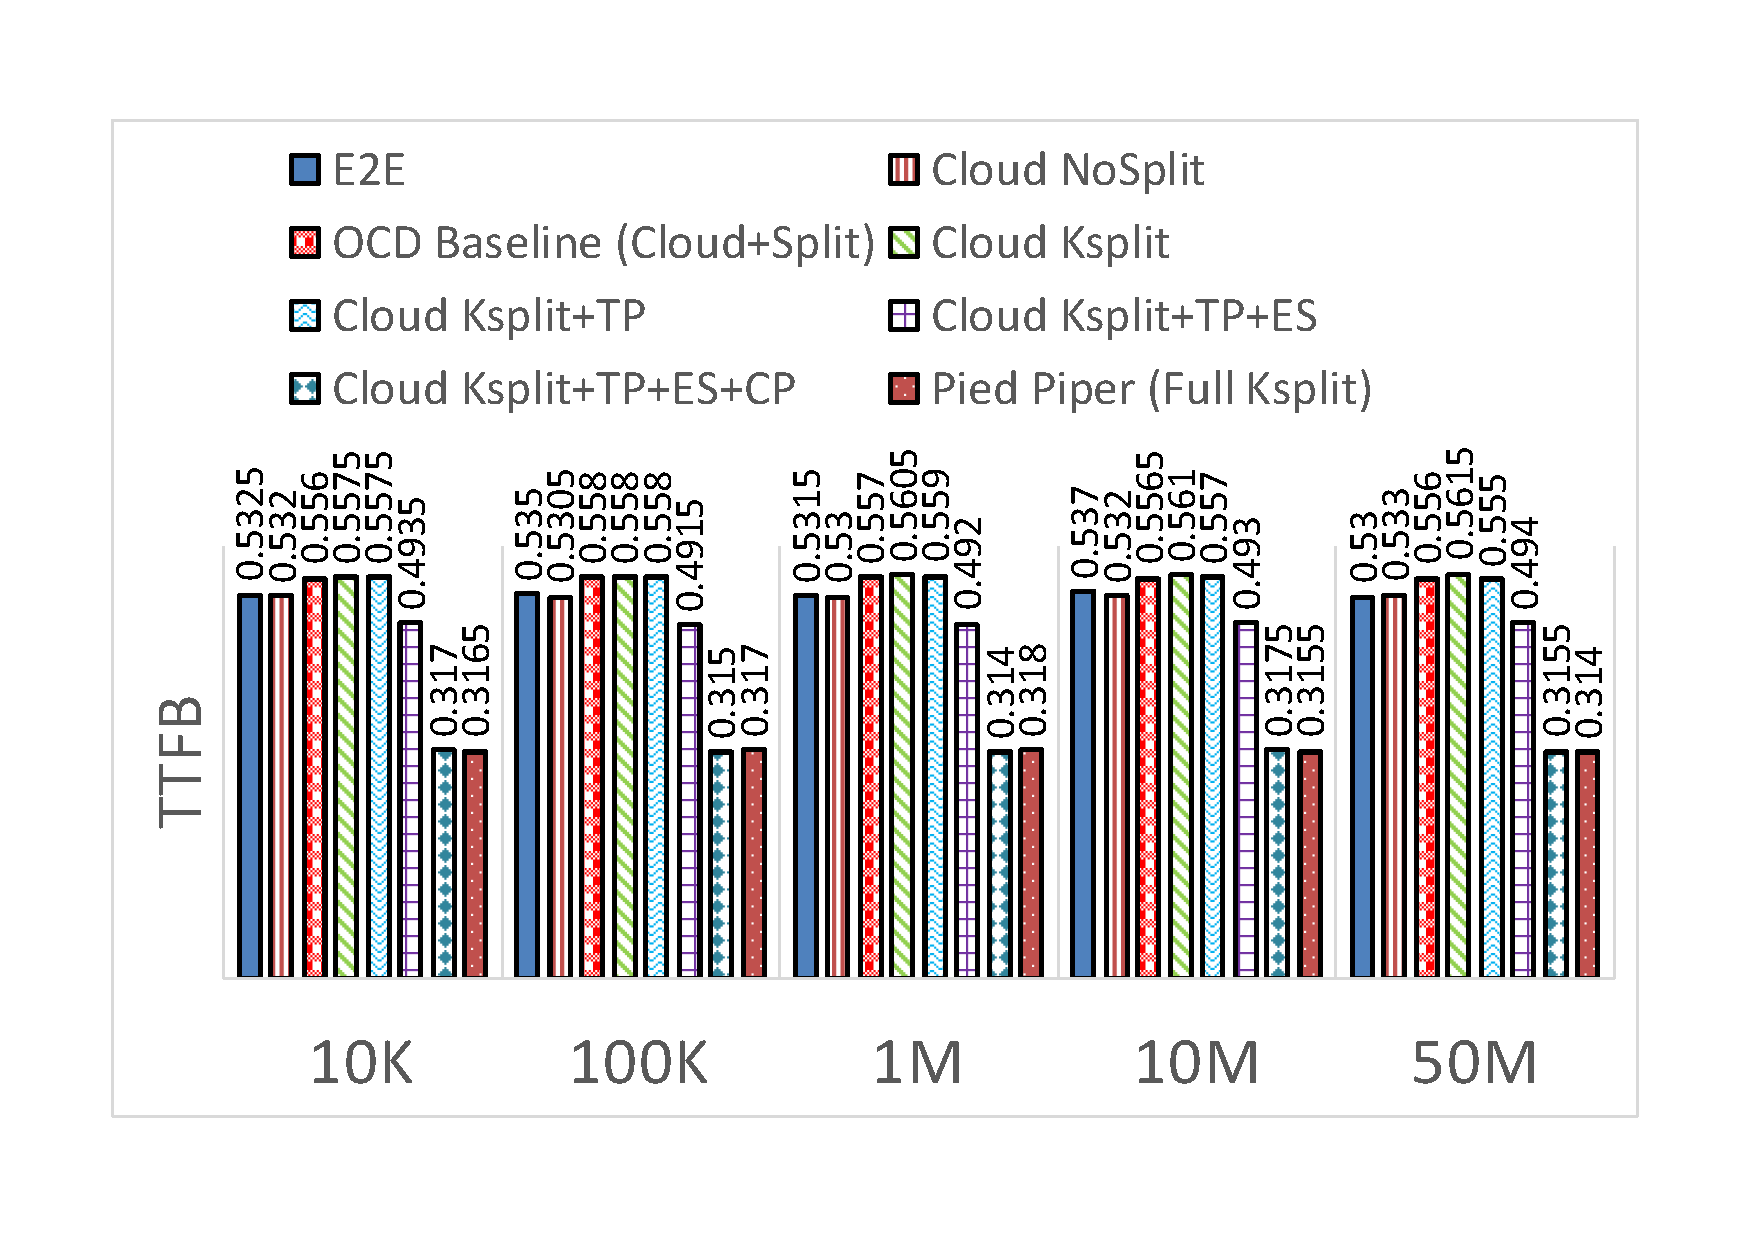
\includegraphics[width=\columnwidth,trim=20mm 25mm 20mm 22mm,clip]{figures/oursys-ttfb.pdf}
    \caption{Time-To-First-Byte (TTFB) in seconds. Median results of 50 runs.}%\AB{Come to think of it, all of these results are basically the same. The TTBF is not suppossed to change between different file sizes, and the results corroborate this. All in favor of just keeping one? pick your favorite :-)} 
    \label{fig:oursys-ttfb}
\end{figure}

\begin{figure}
  \centering
    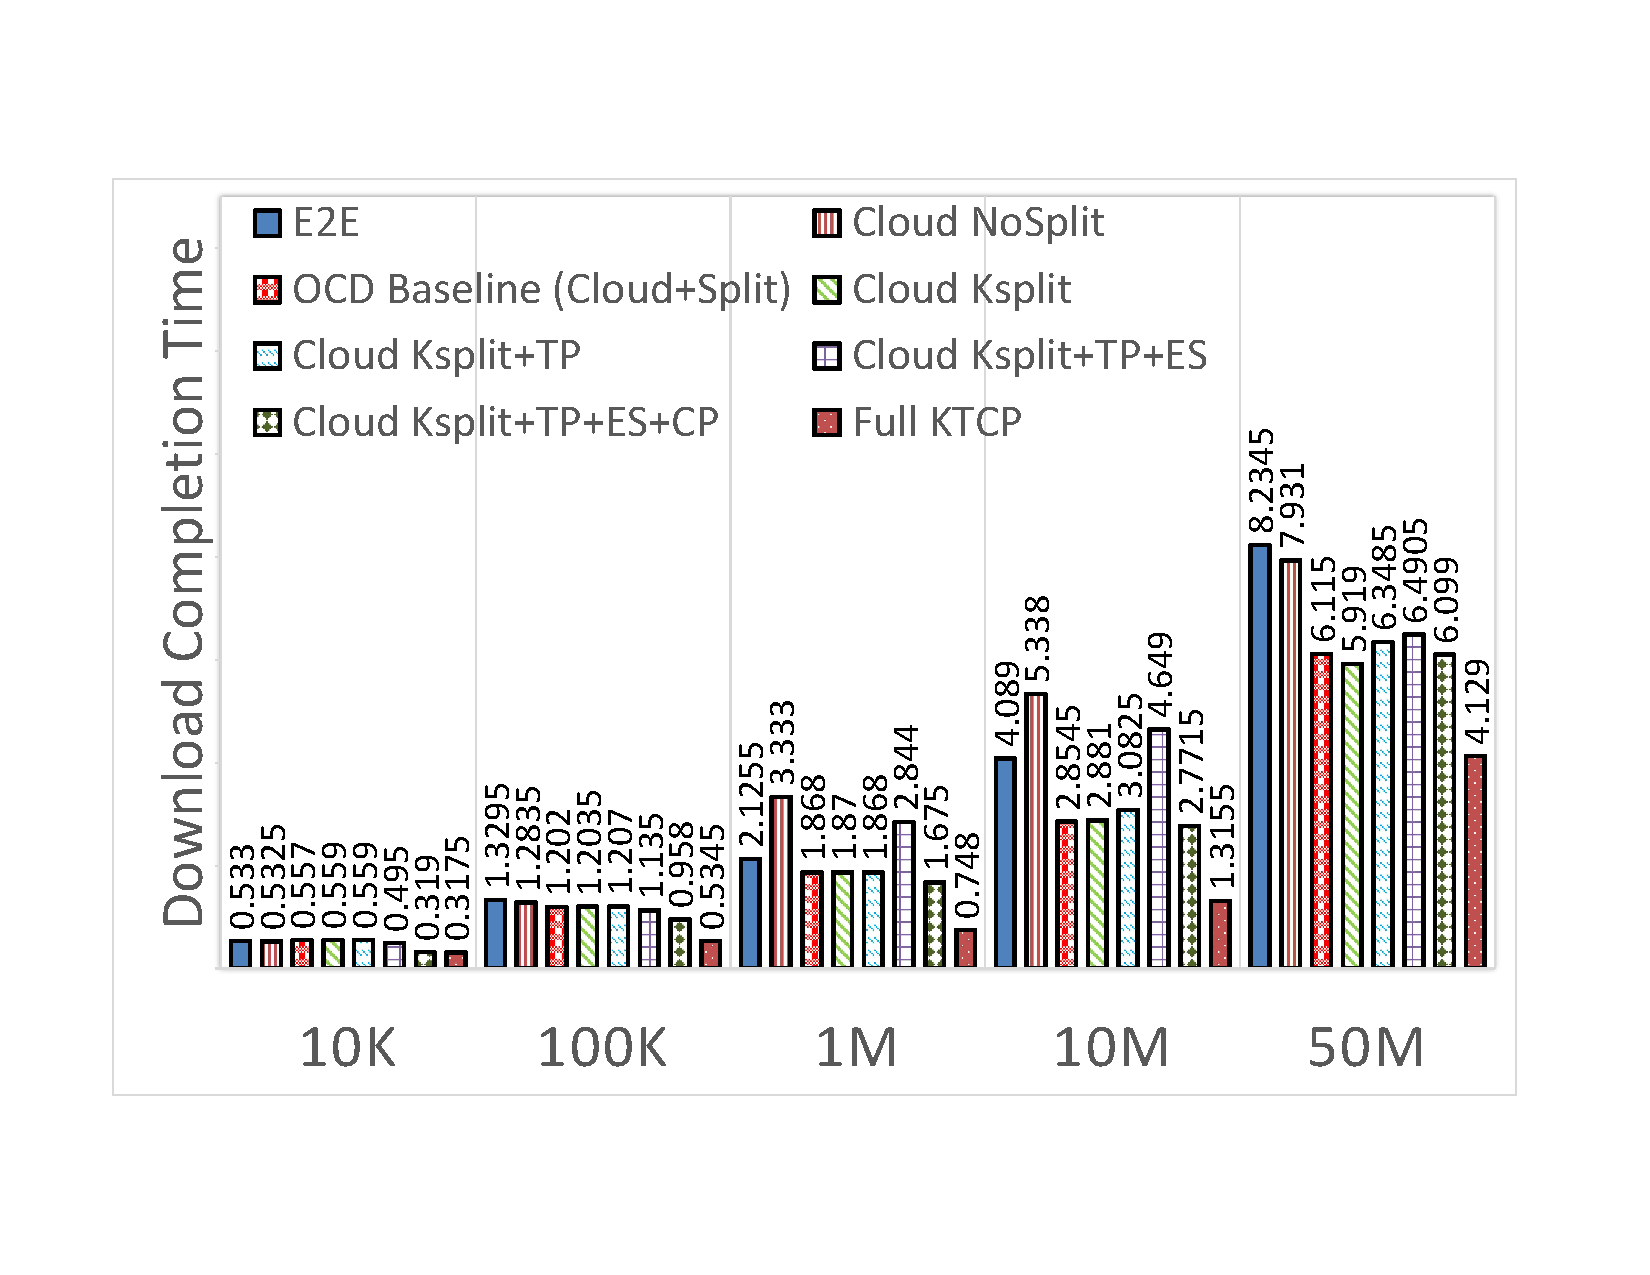
\includegraphics[width=\columnwidth,trim=20mm 25mm 20mm 23mm,clip]{figures/oursys-download.pdf}
    \caption{Download completion time in seconds. Median results of 50 runs.} 
    \label{fig:oursys-download}
\end{figure}




\begin{figure}
  \centering
    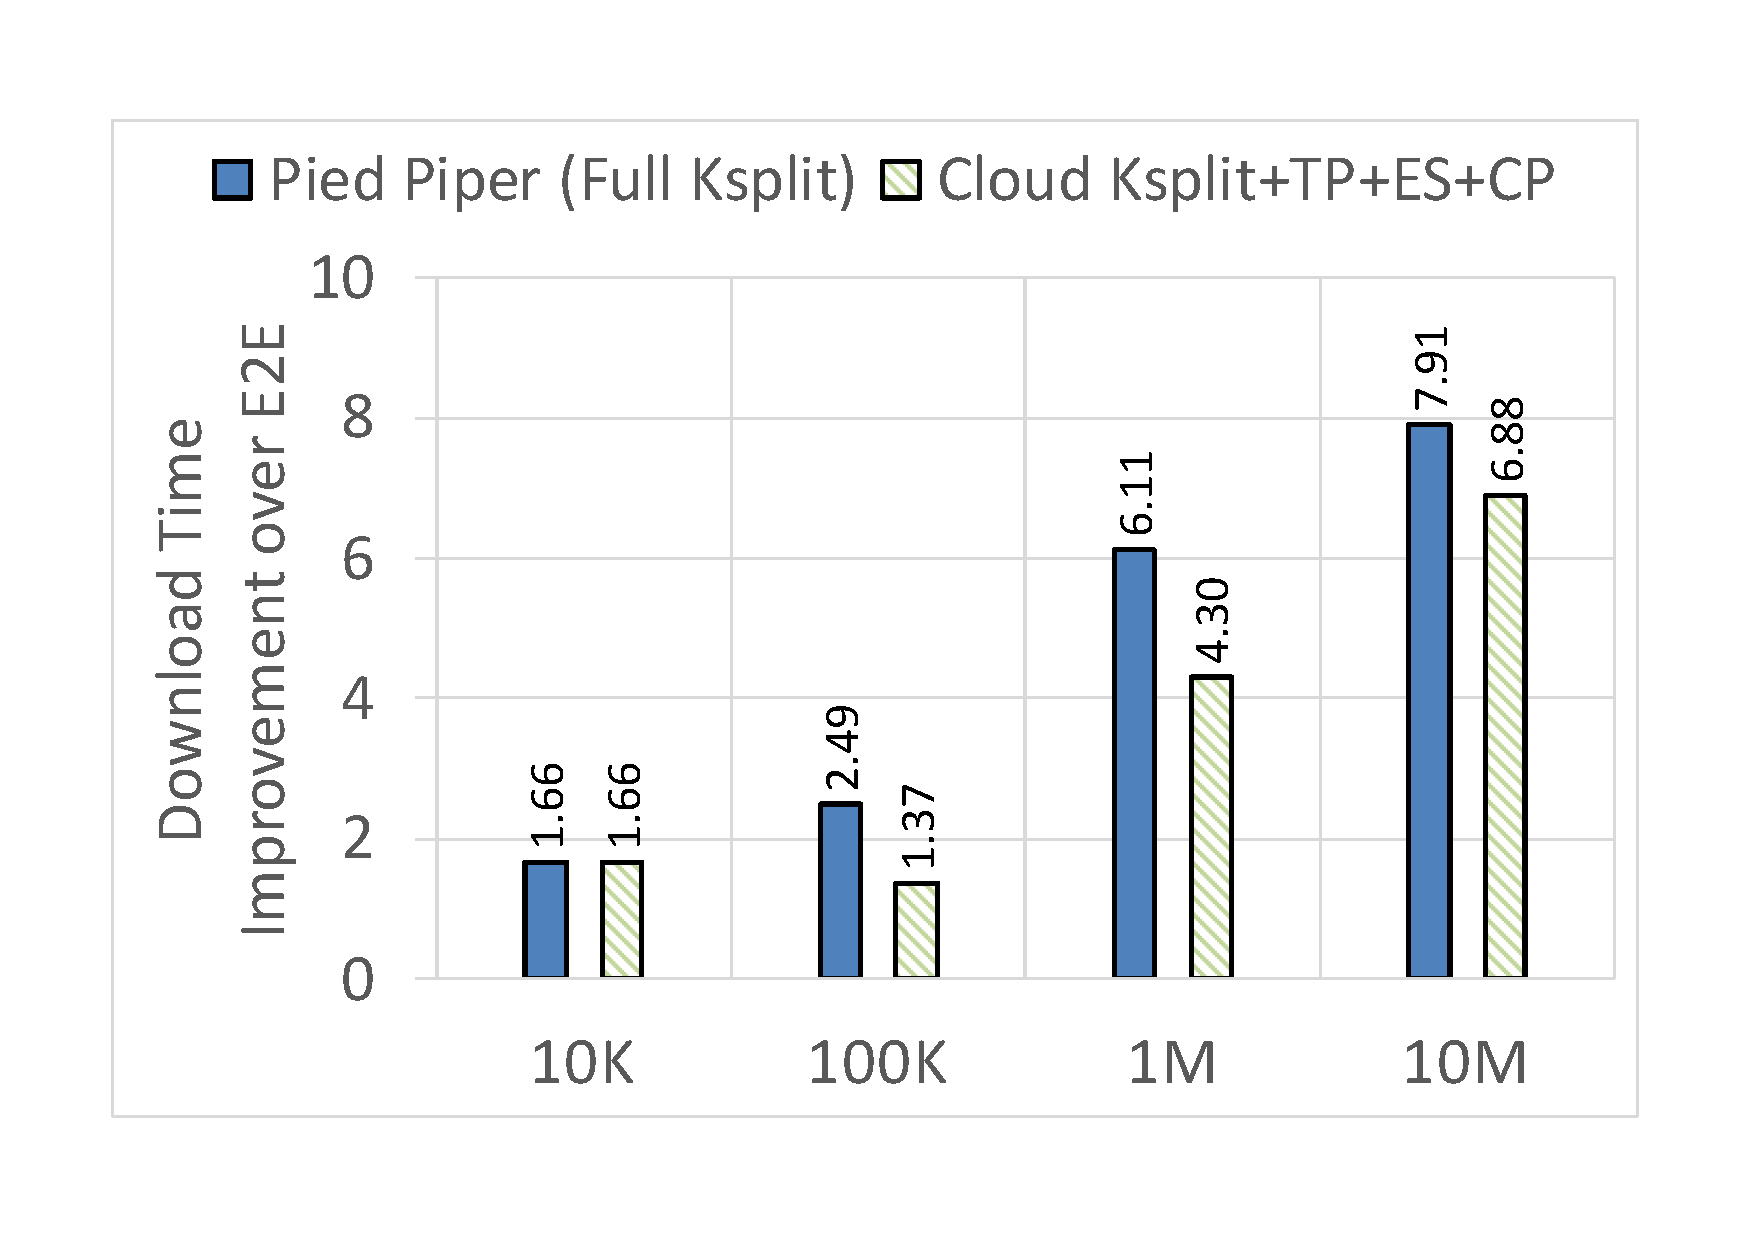
\includegraphics[width=\columnwidth,trim=20mm 25mm 25mm 25mm,clip]{figures/WeakClient-Improvement.pdf}
    \caption{Improvement of \oursys performance over e2e in the case of a memory-limited client. Averaged results over 30 runs.} 
    \label{fig:oursys-weak-client}
\end{figure}

% \section{Routing Strategy}\label{sec:routing-strategy}

% \IK{Do we want to include the results here, or only mention strategies then have an experimental section?}

% 1 vs. 2 vs. 3 relays, intra-cloud vs. multiple clouds, ...


%\IK{Also need to check going through points outside the cloud: here are settings we mentioned:\\
%1. France-Switzerland-Prashanth(SF)-Israel(SF), or\\
%2. France-Switzerland-Amazon(SF)-Israel(SF), \ie half cloud}


\bibliographystyle{acm}
\bibliography{bib,overlaybib,sigcomm18,radio}
\end{document}
